% Figure from MATH 591 notes, section 67. Added, not from lecture: the loop c(t) = (t^2 - 1, t^3 - t) lifted to (point, direction of velocity); the crossing comes apart.
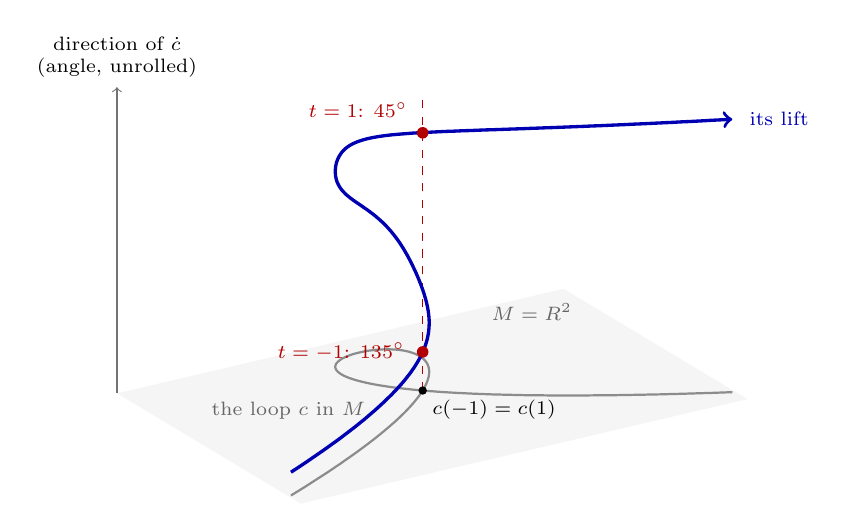
\begin{tikzpicture}[scale=0.95]
\fill[black!4] (-4.087,-0.038) -- (-1.629,-1.512) -- (4.342,-0.115) -- (1.883,1.360) -- cycle;
\node[font=\scriptsize, black!60] at (1.459,1.048) {$M = \mathbb{R}^2$};
\draw[->, black!55] (-4.087,-0.038) -- (-4.087,4.056) node[above, font=\scriptsize, text=black, align=center] {direction of $\dot c$\\ (angle, unrolled)};
\draw[black!45, thick] plot[smooth] coordinates {(-1.761,-1.403) (-1.687,-1.358) (-1.614,-1.313) (-1.544,-1.269) (-1.476,-1.225) (-1.409,-1.182) (-1.344,-1.140) (-1.280,-1.099) (-1.219,-1.058) (-1.159,-1.017) (-1.100,-0.978) (-1.044,-0.938) (-0.989,-0.900) (-0.935,-0.862) (-0.883,-0.825) (-0.833,-0.788) (-0.784,-0.752) (-0.737,-0.717) (-0.692,-0.682) (-0.647,-0.648) (-0.605,-0.614) (-0.564,-0.581) (-0.524,-0.548) (-0.486,-0.516) (-0.449,-0.485) (-0.413,-0.454) (-0.379,-0.424) (-0.346,-0.394) (-0.315,-0.365) (-0.285,-0.336) (-0.256,-0.308) (-0.229,-0.281) (-0.203,-0.254) (-0.178,-0.227) (-0.154,-0.201) (-0.132,-0.176) (-0.111,-0.151) (-0.091,-0.127) (-0.072,-0.103) (-0.054,-0.080) (-0.038,-0.057) (-0.022,-0.034) (-0.008,-0.012) (0.005,0.009) (0.018,0.030) (0.029,0.050) (0.039,0.070) (0.048,0.090) (0.056,0.109) (0.063,0.127) (0.069,0.145) (0.074,0.163) (0.079,0.180) (0.082,0.197) (0.084,0.213) (0.086,0.229) (0.087,0.244) (0.087,0.259) (0.086,0.274) (0.084,0.288) (0.081,0.301) (0.078,0.315) (0.074,0.327) (0.069,0.340) (0.064,0.352) (0.057,0.364) (0.051,0.375) (0.043,0.386) (0.035,0.396) (0.026,0.406) (0.017,0.416) (0.007,0.425) (-0.004,0.434) (-0.015,0.443) (-0.027,0.451) (-0.039,0.459) (-0.052,0.466) (-0.065,0.473) (-0.079,0.480) (-0.093,0.487) (-0.108,0.493) (-0.123,0.499) (-0.138,0.504) (-0.154,0.509) (-0.170,0.514) (-0.187,0.519) (-0.203,0.523) (-0.221,0.527) (-0.238,0.530) (-0.256,0.534) (-0.274,0.537) (-0.292,0.539) (-0.310,0.542) (-0.329,0.544) (-0.348,0.546) (-0.367,0.547) (-0.386,0.548) (-0.406,0.549) (-0.425,0.550) (-0.445,0.551) (-0.464,0.551) (-0.484,0.551) (-0.504,0.551) (-0.523,0.550) (-0.543,0.549) (-0.563,0.548) (-0.583,0.547) (-0.603,0.546) (-0.622,0.544) (-0.642,0.542) (-0.661,0.540) (-0.681,0.538) (-0.700,0.535) (-0.719,0.533) (-0.738,0.530) (-0.757,0.527) (-0.776,0.523) (-0.794,0.520) (-0.812,0.516) (-0.830,0.512) (-0.848,0.508) (-0.865,0.504) (-0.882,0.500) (-0.899,0.495) (-0.916,0.491) (-0.932,0.486) (-0.947,0.481) (-0.963,0.476) (-0.978,0.470) (-0.992,0.465) (-1.006,0.459) (-1.020,0.454) (-1.033,0.448) (-1.045,0.442) (-1.057,0.436) (-1.069,0.430) (-1.080,0.424) (-1.091,0.417) (-1.100,0.411) (-1.110,0.404) (-1.118,0.398) (-1.126,0.391) (-1.134,0.384) (-1.141,0.377) (-1.147,0.370) (-1.152,0.363) (-1.157,0.356) (-1.160,0.349) (-1.164,0.342) (-1.166,0.335) (-1.167,0.327) (-1.168,0.320) (-1.168,0.313) (-1.167,0.305) (-1.165,0.298) (-1.163,0.290) (-1.159,0.283) (-1.155,0.275) (-1.149,0.267) (-1.143,0.260) (-1.135,0.252) (-1.127,0.245) (-1.118,0.237) (-1.107,0.230) (-1.096,0.222) (-1.084,0.214) (-1.070,0.207) (-1.056,0.199) (-1.040,0.192) (-1.023,0.184) (-1.005,0.177) (-0.986,0.169) (-0.966,0.162) (-0.944,0.155) (-0.921,0.147) (-0.897,0.140) (-0.872,0.133) (-0.846,0.126) (-0.818,0.119) (-0.789,0.112) (-0.759,0.105) (-0.727,0.098) (-0.694,0.091) (-0.659,0.084) (-0.624,0.078) (-0.586,0.071) (-0.548,0.065) (-0.508,0.059) (-0.466,0.052) (-0.423,0.046) (-0.379,0.040) (-0.333,0.034) (-0.285,0.029) (-0.236,0.023) (-0.185,0.018) (-0.133,0.012) (-0.079,0.007) (-0.024,0.002) (0.033,-0.003) (0.092,-0.008) (0.152,-0.012) (0.215,-0.017) (0.278,-0.021) (0.344,-0.025) (0.411,-0.029) (0.480,-0.033) (0.551,-0.036) (0.624,-0.040) (0.698,-0.043) (0.774,-0.046) (0.852,-0.049) (0.932,-0.052) (1.014,-0.054) (1.098,-0.056) (1.183,-0.058) (1.271,-0.060) (1.360,-0.062) (1.452,-0.063) (1.545,-0.064) (1.641,-0.065) (1.738,-0.066) (1.838,-0.066) (1.939,-0.066) (2.043,-0.066) (2.149,-0.066) (2.256,-0.065) (2.366,-0.064) (2.479,-0.063) (2.593,-0.062) (2.709,-0.060) (2.828,-0.058) (2.949,-0.056) (3.072,-0.053) (3.197,-0.051) (3.325,-0.047) (3.455,-0.044) (3.587,-0.040) (3.721,-0.036) (3.858,-0.032) (3.997,-0.027) (4.139,-0.022)};
\draw[red!70!black, dashed] (0.000,0.000) -- (0.000,3.946);
\draw[blue!70!black, very thick, ->] plot[smooth] coordinates {(-1.761,-1.092) (-1.687,-1.044) (-1.614,-0.996) (-1.544,-0.949) (-1.476,-0.902) (-1.409,-0.856) (-1.344,-0.811) (-1.280,-0.766) (-1.219,-0.722) (-1.159,-0.679) (-1.100,-0.636) (-1.044,-0.593) (-0.989,-0.551) (-0.935,-0.510) (-0.883,-0.469) (-0.833,-0.428) (-0.784,-0.389) (-0.737,-0.349) (-0.692,-0.310) (-0.647,-0.272) (-0.605,-0.234) (-0.564,-0.197) (-0.524,-0.160) (-0.486,-0.123) (-0.449,-0.087) (-0.413,-0.052) (-0.379,-0.016) (-0.346,0.018) (-0.315,0.053) (-0.285,0.086) (-0.256,0.120) (-0.229,0.153) (-0.203,0.186) (-0.178,0.218) (-0.154,0.250) (-0.132,0.282) (-0.111,0.313) (-0.091,0.344) (-0.072,0.375) (-0.054,0.406) (-0.038,0.436) (-0.022,0.466) (-0.008,0.495) (0.005,0.525) (0.018,0.554) (0.029,0.583) (0.039,0.612) (0.048,0.640) (0.056,0.669) (0.063,0.697) (0.069,0.725) (0.074,0.753) (0.079,0.781) (0.082,0.809) (0.084,0.837) (0.086,0.865) (0.087,0.893) (0.087,0.921) (0.086,0.949) (0.084,0.977) (0.081,1.006) (0.078,1.034) (0.074,1.062) (0.069,1.091) (0.064,1.120) (0.057,1.149) (0.051,1.178) (0.043,1.208) (0.035,1.237) (0.026,1.267) (0.017,1.298) (0.007,1.328) (-0.004,1.359) (-0.015,1.390) (-0.027,1.422) (-0.039,1.453) (-0.052,1.485) (-0.065,1.517) (-0.079,1.549) (-0.093,1.581) (-0.108,1.613) (-0.123,1.645) (-0.138,1.677) (-0.154,1.709) (-0.170,1.741) (-0.187,1.772) (-0.203,1.803) (-0.221,1.834) (-0.238,1.864) (-0.256,1.894) (-0.274,1.923) (-0.292,1.951) (-0.310,1.979) (-0.329,2.006) (-0.348,2.032) (-0.367,2.057) (-0.386,2.082) (-0.406,2.106) (-0.425,2.130) (-0.445,2.152) (-0.464,2.174) (-0.484,2.195) (-0.504,2.215) (-0.523,2.235) (-0.543,2.254) (-0.563,2.272) (-0.583,2.290) (-0.603,2.307) (-0.622,2.324) (-0.642,2.340) (-0.661,2.355) (-0.681,2.370) (-0.700,2.385) (-0.719,2.399) (-0.738,2.413) (-0.757,2.426) (-0.776,2.439) (-0.794,2.452) (-0.812,2.464) (-0.830,2.477) (-0.848,2.489) (-0.865,2.501) (-0.882,2.512) (-0.899,2.524) (-0.916,2.536) (-0.932,2.547) (-0.947,2.559) (-0.963,2.570) (-0.978,2.582) (-0.992,2.594) (-1.006,2.605) (-1.020,2.617) (-1.033,2.629) (-1.045,2.642) (-1.057,2.654) (-1.069,2.667) (-1.080,2.680) (-1.091,2.693) (-1.100,2.707) (-1.110,2.721) (-1.118,2.736) (-1.126,2.750) (-1.134,2.766) (-1.141,2.781) (-1.147,2.797) (-1.152,2.814) (-1.157,2.831) (-1.160,2.848) (-1.164,2.866) (-1.166,2.884) (-1.167,2.902) (-1.168,2.921) (-1.168,2.940) (-1.167,2.959) (-1.165,2.978) (-1.163,2.997) (-1.159,3.017) (-1.155,3.036) (-1.149,3.055) (-1.143,3.074) (-1.135,3.093) (-1.127,3.111) (-1.118,3.129) (-1.107,3.147) (-1.096,3.164) (-1.084,3.181) (-1.070,3.197) (-1.056,3.212) (-1.040,3.227) (-1.023,3.242) (-1.005,3.256) (-0.986,3.269) (-0.966,3.281) (-0.944,3.293) (-0.921,3.305) (-0.897,3.315) (-0.872,3.326) (-0.846,3.335) (-0.818,3.344) (-0.789,3.353) (-0.759,3.361) (-0.727,3.369) (-0.694,3.376) (-0.659,3.383) (-0.624,3.389) (-0.586,3.396) (-0.548,3.401) (-0.508,3.407) (-0.466,3.412) (-0.423,3.417) (-0.379,3.421) (-0.333,3.425) (-0.285,3.429) (-0.236,3.433) (-0.185,3.437) (-0.133,3.441) (-0.079,3.444) (-0.024,3.447) (0.033,3.450) (0.092,3.453) (0.152,3.456) (0.215,3.459) (0.278,3.462) (0.344,3.465) (0.411,3.467) (0.480,3.470) (0.551,3.473) (0.624,3.475) (0.698,3.478) (0.774,3.481) (0.852,3.484) (0.932,3.486) (1.014,3.489) (1.098,3.492) (1.183,3.495) (1.271,3.498) (1.360,3.501) (1.452,3.505) (1.545,3.508) (1.641,3.512) (1.738,3.515) (1.838,3.519) (1.939,3.523) (2.043,3.527) (2.149,3.531) (2.256,3.536) (2.366,3.540) (2.479,3.545) (2.593,3.550) (2.709,3.555) (2.828,3.561) (2.949,3.566) (3.072,3.572) (3.197,3.578) (3.325,3.584) (3.455,3.591) (3.587,3.597) (3.721,3.604) (3.858,3.612) (3.997,3.619) (4.139,3.627)};
\fill (0.000,0.000) circle (1.6pt) node[below right, font=\scriptsize] {$c(-1) = c(1)$};
\fill[red!70!black] (0.000,0.516) circle (2.2pt) node[left=3pt, font=\scriptsize] {$t = -1$: $135^\circ$};
\fill[red!70!black] (0.000,3.445) circle (2.2pt) node[above left=2pt, font=\scriptsize] {$t = 1$: $45^\circ$};
\node[font=\scriptsize, black!60, anchor=west] at (-2.951,-0.267) {the loop $c$ in $M$};
\node[font=\scriptsize, blue!70!black, anchor=west] at (4.239,3.627) {its lift};
\end{tikzpicture}
